Para esta sección, se han elaborado los siguientes diagramas de Gantt relativos a cada uno de los retos a entregrar.

\noindent Relativo al reto/PEC 1 se establece el siguiente diagrama.

\begin{figure}[htp]
    \centering
    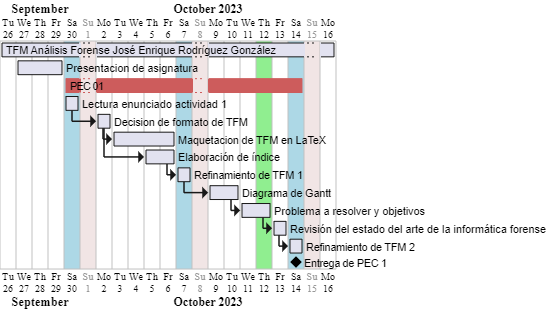
\includegraphics[width=0.8\textwidth]{imagenes/003-diagrama-de-gantt-pec-01.png} 
    \caption{Ejemplo de Diagrama de Gantt relativo al reto/PEC 01.}
    \label{fig:ejemplo_gantt}
\end{figure}

\clearpage

\noindent Relativo al reto/PEC 2 se establece el siguiente diagrama.

\begin{figure}[htp]
    \centering
    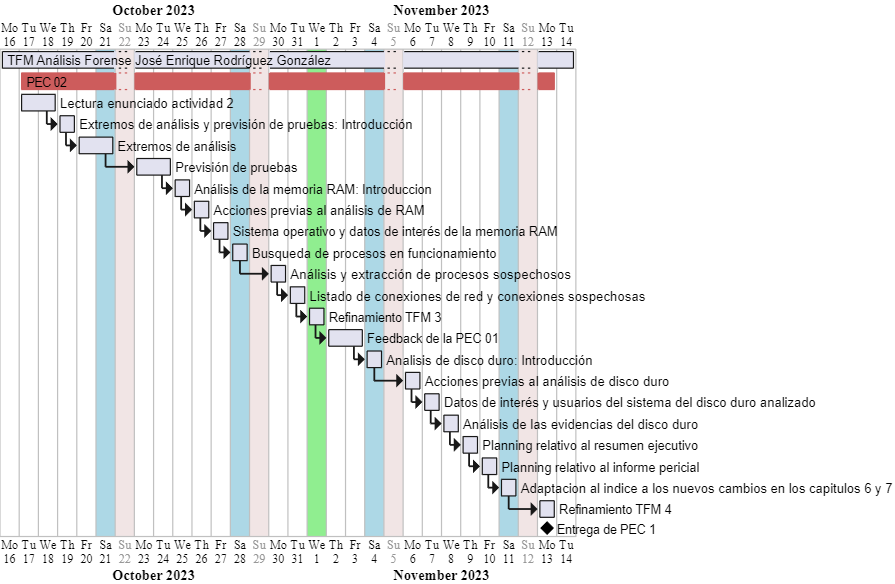
\includegraphics[width=0.8\textwidth]{imagenes/004-diagrama-de-gantt-pec-02.png} 
    \caption{Ejemplo de Diagrama de Gantt relativo al reto/PEC 02.}
    \label{fig:ejemplo_gantt}
\end{figure}

\clearpage

\noindent Relativo al reto/PEC 3 se establece el siguiente diagrama.

\begin{figure}[htp]
    \centering
    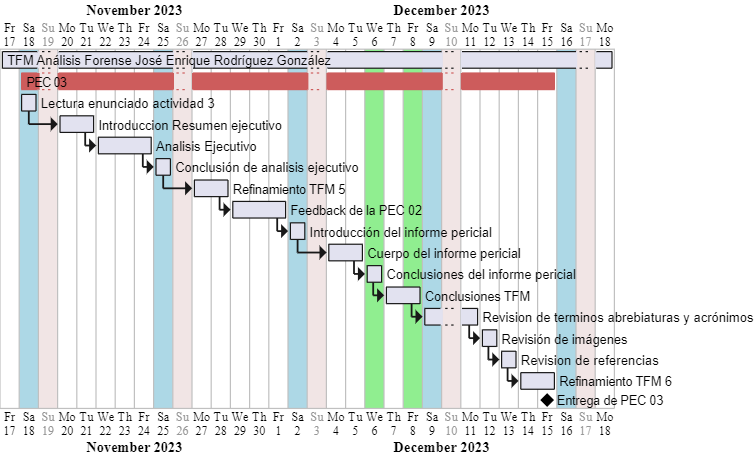
\includegraphics[width=0.8\textwidth]{imagenes/005-diagrama-de-gantt-pec-03.png} 
    \caption{Ejemplo de Diagrama de Gantt relativo al reto/PEC 03.}
    \label{fig:ejemplo_gantt}
\end{figure}


\clearpage

\noindent Relativo al reto/PEC 4 se establece el siguiente diagrama.

\begin{figure}[htp]
    \centering
    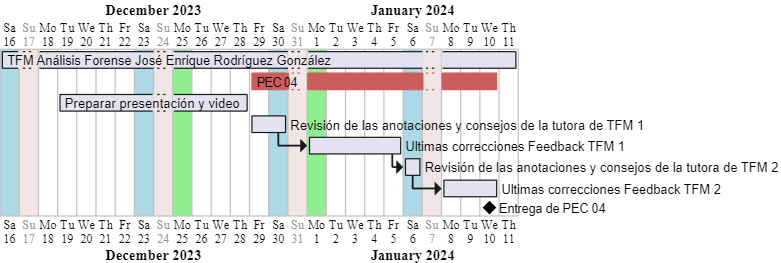
\includegraphics[width=0.8\textwidth]{imagenes/006-diagrama-de-gantt-pec-04.png} 
    \caption{Ejemplo de Diagrama de Gantt relativo al reto/PEC 04.}
    \label{fig:ejemplo_gantt}
\end{figure}

